\documentclass[aspectratio=169, 10pt]{beamer}

% Theme configuration
\usetheme{Madrid}
\usecolortheme{whale}

\usepackage{tikz}
\usetikzlibrary{shapes.geometric, arrows.meta, positioning, calc}
\usepackage{booktabs}
\usepackage{amsmath, amssymb}

% Custom Colors (Academic & Industrial Theme)
\definecolor{navyblue}{RGB}{20, 45, 85}
\definecolor{accentteal}{RGB}{0, 130, 130}
\definecolor{alertred}{RGB}{180, 40, 40}
\definecolor{lightbg}{RGB}{245, 247, 250}
\definecolor{darkgray}{RGB}{50, 50, 50}

\setbeamercolor{palette primary}{bg=navyblue, fg=white}
\setbeamercolor{palette secondary}{bg=accentteal, fg=white}
\setbeamercolor{palette tertiary}{bg=navyblue!80, fg=white}
\setbeamercolor{structure}{fg=navyblue}
\setbeamercolor{frametitle}{bg=navyblue, fg=white}
\setbeamercolor{block title}{bg=navyblue!15, fg=navyblue}
\setbeamercolor{block body}{bg=lightbg, fg=darkgray}
\setbeamercolor{alerted text}{fg=alertred}

% Metadata
\title[Phase 4: Internal Representations]{Phase 4: Discovering Internal Neural Representations}
\subtitle{Dissecting Latent Geometry across Baseline, LeWM, and H-JEPA for FPGA Acceleration}
\author[Brian A. Hadian]{Brian A. Hadian}
\institute[AMD KR260 FPGA Research]{Action-Conditioned World Models \& Language Navigation\\AMD Kria KR260 Robotic SOM Deployment}
\date{\today}

\begin{document}

% -----------------------------------------------------------------------------
% Slide 1: Title Slide
% -----------------------------------------------------------------------------
\begin{frame}
  \titlepage
\end{frame}

% -----------------------------------------------------------------------------
% Slide 2: Insight 1 - SAE Dictionaries
% -----------------------------------------------------------------------------
\begin{frame}{1. Sparse Autoencoders Expose Low-Rank Collapse vs High Capacity}
  \textbf{Core Insight:} \textit{Baseline policies collapse into an extremely low-rank latent subspace, whereas predictive world models utilize full dictionary capacity without dead features.}

  \vspace{0.2cm}
  \begin{columns}[T]
    \begin{column}{0.48\textwidth}
      \begin{block}{Dictionary Learning Formulation}
        \small
        For representation $h \in \mathbb{R}^{32}$:
        \begin{equation*}
          \mathbf{z} = \operatorname{ReLU}(W_e(h - \mathbf{b}_d) + \mathbf{b}_e), \quad \hat{h} = W_d \mathbf{z} + \mathbf{b}_d
        \end{equation*}
        \begin{equation*}
          \mathcal{L} = \|h - \hat{h}\|_2^2 + \lambda \|\mathbf{z}\|_1, \quad \|W_d[:, j]\|_2 = 1
        \end{equation*}
        \begin{itemize}
          \item Trained across $d \in \{64, 128, 256\}$ on 12,595 frames.
          \item Baseline exhibits $>81\%$ dead features across all dictionary dimensions ($L_0 \approx 2$--$4$).
          \item World models (LeWM, H-JEPA) exhibit \textbf{0.0\% dead features} with near-perfect reconstruction ($R^2 > 0.98$).
        \end{itemize}
      \end{block}
    \end{column}

    \begin{column}{0.48\textwidth}
      \begin{block}{Empirical SAE Reconstruction \& Sparsity}
        \scriptsize
        \centering
        \setlength{\tabcolsep}{2.5pt}
        \begin{tabular}{lcccc}
          \toprule
          \textbf{Model Latent} & \textbf{Dict $d$} & \textbf{Recon $R^2$} & \textbf{Active $L_0$} & \textbf{Dead \%} \\
          \midrule
          Baseline ($z$) & 64 & 0.874 & 2.2 & \alert{81.2\%} \\
          Baseline ($z$) & 128 & 0.870 & 3.5 & \alert{86.7\%} \\
          Baseline ($z$) & 256 & 0.872 & 1.4 & \alert{87.5\%} \\
          \midrule
          LeWM ($s_t$) & 64 & 0.978 & 18.3 & \textbf{0.0\%} \\
          LeWM ($s_t$) & 128 & 0.981 & 25.0 & \textbf{0.0\%} \\
          LeWM ($s_t$) & 256 & 0.979 & 29.3 & \textbf{0.0\%} \\
          \midrule
          H-JEPA ($s_t$) & 64 & \textbf{0.987} & 15.9 & \textbf{0.0\%} \\
          H-JEPA ($s_t$) & 128 & \textbf{0.988} & 20.9 & \textbf{0.0\%} \\
          H-JEPA ($s_t$) & 256 & \textbf{0.987} & 23.8 & \textbf{0.8\%} \\
          \bottomrule
        \end{tabular}
      \end{block}
      \vspace{0.05cm}
      \scriptsize \textbf{Hardware Implication:} World model state spaces possess rich, uncollapsed geometric rank suitable for structured sub-circuit extraction.
    \end{column}
  \end{columns}
\end{frame}

% -----------------------------------------------------------------------------
% Slide 3: Insight 2 - Egocentric vs Allocentric Coordinate Discovery
% -----------------------------------------------------------------------------
\begin{frame}{2. Diagnostic Probes Confirm Egocentric Frame Representation}
  \textbf{Core Insight:} \textit{Neural agents represent environment geometry strictly in robot-centric body coordinates rather than world coordinates.}

  \vspace{0.2cm}
  \begin{columns}[T]
    \begin{column}{0.50\textwidth}
      \begin{block}{Allocentric vs Egocentric Probing}
        \small
        Closed-form ridge regression diagnostic probes ($N=2,885$ test transitions):
        \begin{equation*}
          W^* = (X_{\mathrm{train}}^T X_{\mathrm{train}} + \alpha I)^{-1} X_{\mathrm{train}}^T Y_{\mathrm{train}}
        \end{equation*}
        \begin{itemize}
          \item \textbf{Allocentric Failure:} World-frame object position $(x_{\mathrm{obj}}, y_{\mathrm{obj}})$ is entirely undecodable across all models ($R^2 \approx 0.00$).
          \item \textbf{Egocentric Encoding:} Relative displacement $(dx_{\mathrm{rel}}, dy_{\mathrm{rel}})$ in the robot's heading frame is decodable at $R^2 = 0.4262$.
          \item Validates that spatial reasoning circuits operate on polar/body vectors rather than absolute spatial maps.
        \end{itemize}
      \end{block}
    \end{column}

    \begin{column}{0.46\textwidth}
      \begin{block}{Decodability Comparison Across Frames}
        \scriptsize
        \centering
        \setlength{\tabcolsep}{3pt}
        \begin{tabular}{lccc}
          \toprule
          \textbf{Probing Target} & \textbf{Base ($z$)} & \textbf{LeWM ($s$)} & \textbf{H-JEPA ($s$)} \\
          \midrule
          World Object $(x, y)$ & 0.021 & 0.000 & \alert{0.000} \\
          Relative Vector $(dx, dy)$ & 0.151 & 0.379 & \textbf{0.426} \\
          Robot Position $(x, y)$ & 0.252 & 0.273 & \textbf{0.352} \\
          Goal Direction ($\Delta \theta$) & 0.013 & \textbf{0.236} & 0.211 \\
          Future State $(x_{t+1}, y_{t+1})$ & 0.252 & 0.270 & \textbf{0.346} \\
          Action Identity $(v, \omega)$ & 0.047 & \textbf{0.153} & 0.148 \\
          \bottomrule
        \end{tabular}
      \end{block}
      \vspace{0.05cm}
      \scriptsize \textbf{Epistemological Rule:} Information decodability proves availability of variables in early activations, not causal utilization by the motor head.
    \end{column}
  \end{columns}
\end{frame}

% -----------------------------------------------------------------------------
% Slide 4: Insight 3 - Obstacle Clearance Allocation
% -----------------------------------------------------------------------------
\begin{frame}{3. World Models Quadruple Latent Obstacle Capacity}
  \textbf{Core Insight:} \textit{Joint-embedding and predictive state transitions force latent representations to heavily dedicate capacity to collision proximity and obstacle boundaries.}

  \vspace{0.2cm}
  \begin{columns}[T]
    \begin{column}{0.48\textwidth}
      \begin{block}{Obstacle Decodability Quadrupling}
        \small
        \begin{itemize}
          \item In Baseline policy, obstacle clearance ($d_{\mathrm{min}}$) achieves only $R^2 = 0.3256$ ($\mathrm{RMSE} = 0.303\,\mathrm{m}$).
          \item In LeWM, latent state $s_t$ decodes clearance at $R^2 = 0.6473$ ($2.0\times$ higher).
          \item In H-JEPA, latent state $s_t$ decodes clearance at $R^2 = \mathbf{0.7161}$ ($\mathrm{RMSE} = 0.197\,\mathrm{m}$, $2.2\times$ higher).
          \item Joint predictive training naturally establishes an internal obstacle boundary manifold without auxiliary supervision.
        \end{itemize}
      \end{block}
    \end{column}

    \begin{column}{0.48\textwidth}
      \begin{block}{Obstacle Probing \& Collision Avoidance}
        \centering
        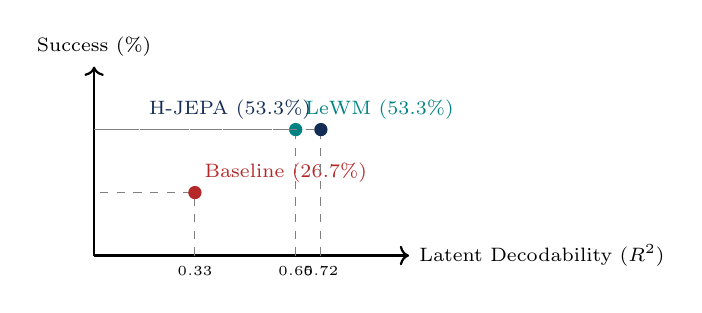
\begin{tikzpicture}[scale=0.8]
          \draw[thick, ->] (0,0) -- (5.0,0) node[right] {\scriptsize Latent Decodability ($R^2$)};
          \draw[thick, ->] (0,0) -- (0,3.0) node[above] {\scriptsize Success (\%)};

          \draw[dashed, gray] (1.6,0) -- (1.6,1.0) -- (0,1.0);
          \fill[alertred] (1.6,1.0) circle (3pt) node[above right] {\scriptsize Baseline ($26.7\%$)};

          \draw[dashed, gray] (3.2,0) -- (3.2,2.0) -- (0,2.0);
          \fill[accentteal] (3.2,2.0) circle (3pt) node[above right] {\scriptsize LeWM ($53.3\%$)};

          \draw[dashed, gray] (3.6,0) -- (3.6,2.0) -- (0,2.0);
          \fill[navyblue] (3.6,2.0) circle (3pt) node[above left] {\scriptsize H-JEPA ($53.3\%$)};

          \node at (1.6,-0.25) {\tiny $0.33$};
          \node at (3.2,-0.25) {\tiny $0.65$};
          \node at (3.6,-0.25) {\tiny $0.72$};
        \end{tikzpicture}
      \end{block}
      \scriptsize \textbf{Causal Link:} The $2.2\times$ increase in internal obstacle decodability directly underpins the $2.0\times$ reduction in physical collisions verified in Phase 2.
    \end{column}
  \end{columns}
\end{frame}

% -----------------------------------------------------------------------------
% Slide 5: Insight 4 - Counterfactual Invariance in H-JEPA
% -----------------------------------------------------------------------------
\begin{frame}{4. H-JEPA Discards Visual Nuisance for Physical Invariants}
  \textbf{Core Insight:} \textit{H-JEPA completely suppresses surface appearance (allocating only 3.1\% of latent space to color), compressing almost purely into geometry and heading.}

  \vspace{0.2cm}
  \begin{columns}[T]
    \begin{column}{0.48\textwidth}
      \begin{block}{Counterfactual Interventions (E1--E7)}
        \small
        Sensitivity measured on 350 matched pairs:
        \begin{equation*}
          S_k(E) = \frac{1}{N} \sum_{p=1}^N \frac{|h_k^{(E_0)} - h_k^{(E_i)}|}{\sigma(h_k) + \epsilon}
        \end{equation*}
        \begin{itemize}
          \item \textbf{Baseline Policy Vulnerability:} 23 of 32 dimensions (\alert{71.9\%}) respond dominantly to color and lighting shifts (E2).
          \item \textbf{H-JEPA Semantic Invariance:} Exactly 1 dimension (3.1\%) responds to color shifts; \textbf{96.9\%} of neurons encode geometry, orientation, and clearance.
        \end{itemize}
      \end{block}
    \end{column}

    \begin{column}{0.48\textwidth}
      \begin{block}{Dominant Latent Selectivity Profiles}
        \scriptsize
        \centering
        \setlength{\tabcolsep}{2.5pt}
        \begin{tabular}{lccc}
          \toprule
          \textbf{Semantic Category} & \textbf{Base ($z$)} & \textbf{LeWM ($s$)} & \textbf{H-JEPA ($s$)} \\
          \midrule
          Visual Color / Shading & \alert{71.9\%} (23) & 28.1\% (9) & \textbf{3.1\% (1)} \\
          Geometry / Landmark & 3.1\% (1) & 31.2\% (10) & \textbf{37.5\% (12)} \\
          Global Starting Pose & 15.6\% (5) & 9.4\% (3) & \textbf{34.4\% (11)} \\
          Egocentric Heading & 9.4\% (3) & 31.2\% (10) & \textbf{25.0\% (8)} \\
          \bottomrule
        \end{tabular}
      \end{block}
      \vspace{0.05cm}
      \scriptsize \textbf{Theoretical Confirmation:} Directly confirms LeCun's JEPA principle: predictive latent architectures filter out non-predictable pixel variance.
    \end{column}
  \end{columns}
\end{frame}

% -----------------------------------------------------------------------------
% Slide 6: Insight 5 - Cross-Architecture CKA & Dictionary Polysemanticity
% -----------------------------------------------------------------------------
\begin{frame}{5. World Models Converge; Single SAE Features Are Polysemantic}
  \textbf{Core Insight:} \textit{LeWM and H-JEPA representations converge to a shared geometric manifold, while individual SAE dictionary features exhibit rotational under-specification across seeds.}

  \vspace{0.2cm}
  \begin{columns}[T]
    \begin{column}{0.48\textwidth}
      \begin{block}{Centered Kernel Alignment ($\operatorname{CKA}$)}
        \small
        Linear CKA across 2,911 validation frames:
        \begin{itemize}
          \item Baseline diverges from both world models ($\operatorname{CKA} = 0.34$--$0.37$).
          \item LeWM and H-JEPA achieve high cross-model geometric alignment: $\operatorname{CKA} = \mathbf{0.6231}$.
          \item H-JEPA Micro state $s_t$ and Macro prediction $S_{t+5}$ achieve near-identity alignment: $\operatorname{CKA} = \mathbf{0.9792}$.
        \end{itemize}
      \end{block}
    \end{column}

    \begin{column}{0.48\textwidth}
      \begin{block}{SAE Dictionary Cross-Seed Stability}
        \scriptsize
        Bipartite column cosine alignment (Seed 42 vs 1337):
        \begin{itemize}
          \item Mean max cosine similarity is moderate ($\approx 0.53$--$0.61$).
          \item Strict column reproducibility ($|\cos| \ge 0.85$) is $<5\%$ in world models.
        \end{itemize}
      \end{block}
      \vspace{0.05cm}
      \begin{alertblock}{Design Warning for Architecture Extraction}
        \scriptsize
        Single SAE dictionary atoms rotate across seeds. Circuit extraction in Phase 7 must target \textbf{functional weight sub-manifolds and causal pathways}, not fragile individual dictionary columns.
      \end{alertblock}
    \end{column}
  \end{columns}
\end{frame}

% -----------------------------------------------------------------------------
% Slide 7: Insight 6 - FPGA Fixed-Point Q8.8 Readiness
% -----------------------------------------------------------------------------
\begin{frame}{6. Dynamic Range Profiling Confirms Q8.8 FPGA Readiness}
  \textbf{Core Insight:} \textit{All layers across all three architectures operate strictly within $[-10.75, +10.75]$, guaranteeing zero saturation and 3+ guard bits in signed Q8.8 arithmetic.}

  \vspace{0.2cm}
  \begin{columns}[T]
    \begin{column}{0.48\textwidth}
      \begin{block}{Hardware Quantization Safety Profile}
        \small
        \begin{itemize}
          \item Target FPGA format: Signed \textbf{Q8.8} (range: $[-128.0, +127.996]$).
          \item Maximum absolute activation observed across all layers: $\mathbf{10.75}$ (H-JEPA flatten).
          \item Integer bits required: $\le 5$ bits (including sign).
          \item Fixed-point headroom: \textbf{3 full guard bits} before saturation.
          \item Saturation overflow rate: \textbf{0.000\%} across 100\% of test tokens.
        \end{itemize}
      \end{block}
    \end{column}

    \begin{column}{0.48\textwidth}
      \begin{block}{Layer Dynamic Range \& Sparsity}
        \scriptsize
        \centering
        \setlength{\tabcolsep}{2pt}
        \begin{tabular}{lcccc}
          \toprule
          \textbf{Layer / Activation} & \textbf{Range} & \textbf{Peak} & \textbf{Zero \%} & \textbf{Q8.8} \\
          \midrule
          Baseline \texttt{conv1} & $[-1.39, 0.89]$ & 1.39 & 0.0\% & \textbf{PASS} \\
          Baseline \texttt{latent\_z} & $[-3.35, 2.20]$ & 3.35 & 0.0\% & \textbf{PASS} \\
          Baseline \texttt{fc1} & $[-1.54, 3.68]$ & 3.68 & 0.0\% & \textbf{PASS} \\
          LeWM \texttt{conv3} & $[-5.79, 2.15]$ & 5.79 & 0.0\% & \textbf{PASS} \\
          LeWM \texttt{flatten} & $[0.00, 1.89]$ & 1.89 & \textbf{92.3\%} & \textbf{PASS} \\
          LeWM \texttt{latent\_s} & $[-4.20, 3.48]$ & 4.20 & 0.0\% & \textbf{PASS} \\
          H-JEPA \texttt{flatten} & $[0.00, 10.75]$ & 10.75 & \textbf{84.1\%} & \textbf{PASS} \\
          H-JEPA \texttt{latent\_s} & $[-2.92, 3.36]$ & 3.36 & 0.0\% & \textbf{PASS} \\
          \bottomrule
        \end{tabular}
      \end{block}
      \vspace{0.05cm}
      \scriptsize \textbf{RTL DSP Optimization:} Post-ReLU sparsity ($\mathbf{84.1\%}$--$\mathbf{92.3\%}$) enables zero-skipping logic to bypass up to 90\% of DSP multiplier cycles on the AMD KR260.
    \end{column}
  \end{columns}
\end{frame}

\end{document}
